\chapter{Технологический раздел}

\section{Язык программирования}
В качестве языка программирований выбран язык высокого уровня JavaScript.

\section{Примеры кода}

\begin{lstlisting}[caption={Реализация имитационной модели}]
  while (amountOutput < aBuyer.amount) {

    if (buyer.isRequest(nowTime)) {

      let numberCashier = 0;
      let pollCashiers;

      if (buyer.getWeightReq() <= cashier_fast.max_weight) {
        pollCashiers = fastCashiers;
      } else {
        pollCashiers = cashiers;
      }

      pollCashiers.forEach(function(item, i, arr) {
        if (item.getlengthQueue() < arr[numberCashier].getlengthQueue()) {
          numberCashier = i;
        }
      })
      pollCashiers[numberCashier].pushWork(nowTime, buyer.getWeightReq())

      
      buyer.reset();
  
      ++amountInput;
    }

    fastCashiers.forEach(function(el) {
      amountOutput += el.check(nowTime);
    })

    cashiers.forEach(function(el) {
      amountOutput += el.check(nowTime);
    })

    nowTime += simulator.dt;
  }
\end{lstlisting}

\begin{lstlisting}[caption={Программная модель кассы}]
function ServiceUnit(timePerRequest) {
  let self = this;
  
  self.queue = [];
  self.tpr = timePerRequest;

  let timeNewWork;

  self.getlengthQueue = function() {
    return self.queue.length;
  }

  self.check = function(nowTime) {
    if (self.queue.length == 0) return 0;

    let finished

    if (nowTime >= timeNewWork) {
      finished = self.queue.shift()
    }

    if (finished)  {
      timeNewWork = nowTime + self.queue[0] * self.tpr;
      return 1
    }

    return 0;
  }

  self.pushWork = function(nowTime, weight) {
    if (self.queue.length == 0) 
      timeNewWork = nowTime + weight * self.tpr;

    self.queue.push(weight)
  }
} 
\end{lstlisting}

\begin{lstlisting}[caption={Программная модель покупателя}]
function SourceOfInformation(timeReq, weightReq) {
  let self = this;
  
  self.timeReq = timeReq;
  self.weightReq = weightReq;

  let isRequest = false;

  let timeNewRequest = self.timeReq.randFunc(self.timeReq.param);
  
  let weightNewRequest = self.weightReq.randFunc(self.weightReq.param);

  self.isRequest = function(nowTime) {
    if (nowTime >= timeNewRequest && !isRequest)  {
      isRequest = true;
      timeNewRequest += self.timeReq.randFunc(self.timeReq.param);
      weightNewRequest = self.weightReq.randFunc(self.weightReq.param);
    }

    return isRequest;
  }

  self.getWeightReq = function() {
    return weightNewRequest;
  }

  self.reset = function() {
    isRequest = false;
  }
}
\end{lstlisting}


\section{Взаимодействие с пользователем}

Взаимодейсвтие с пользователем осуществляется через html страницы, открытые в браузере.

\begin{figure}
  \centering
  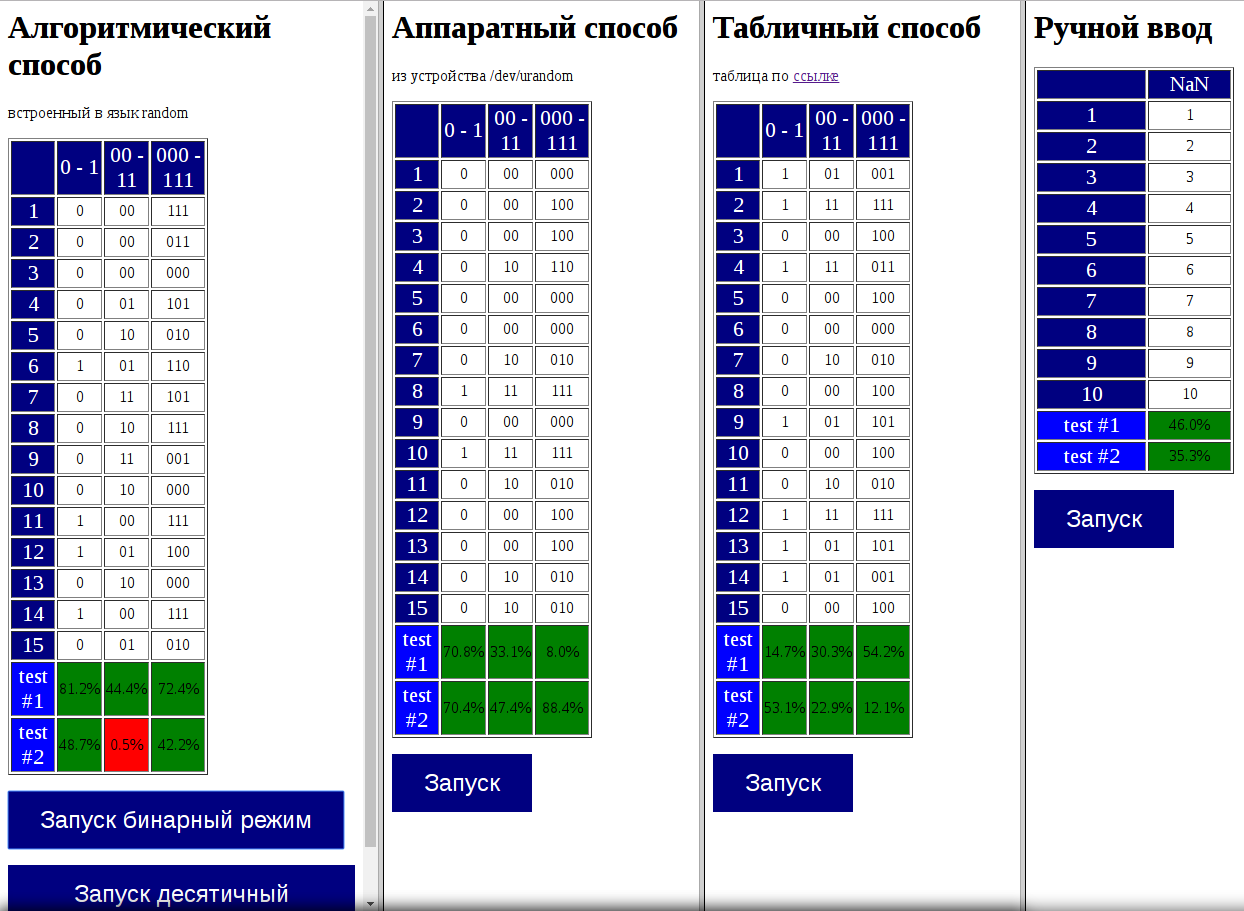
\includegraphics[scale=0.8]{screen1.png}
  \caption{Настройка параметров модели}
\end{figure}

\begin{figure}
  \centering
  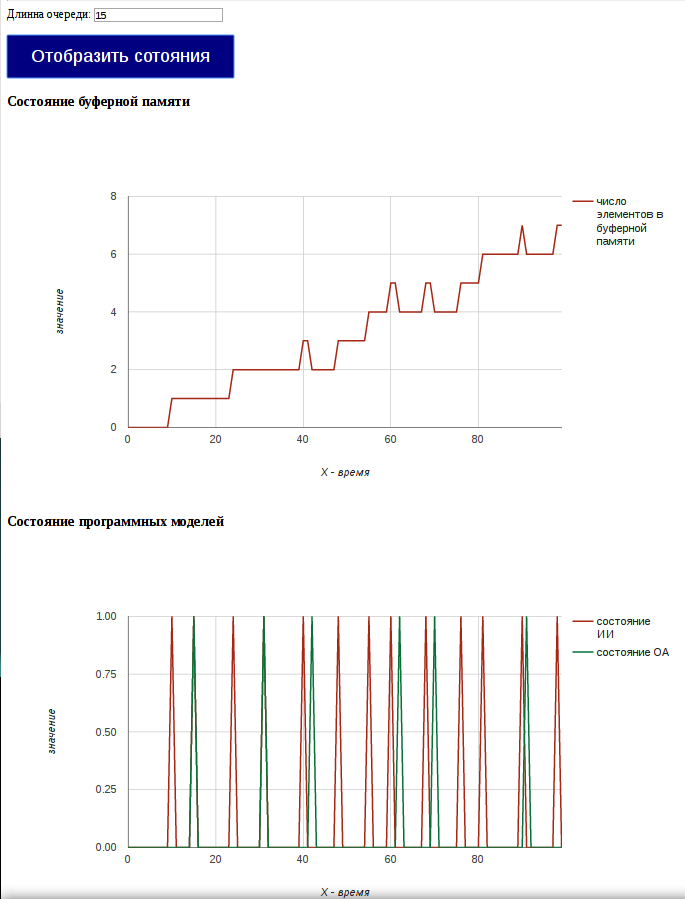
\includegraphics[scale=0.6]{screen2.png}
  \caption{Длинна очереди в каждой быстрой кассе}
\end{figure}

\begin{figure}
  \centering
  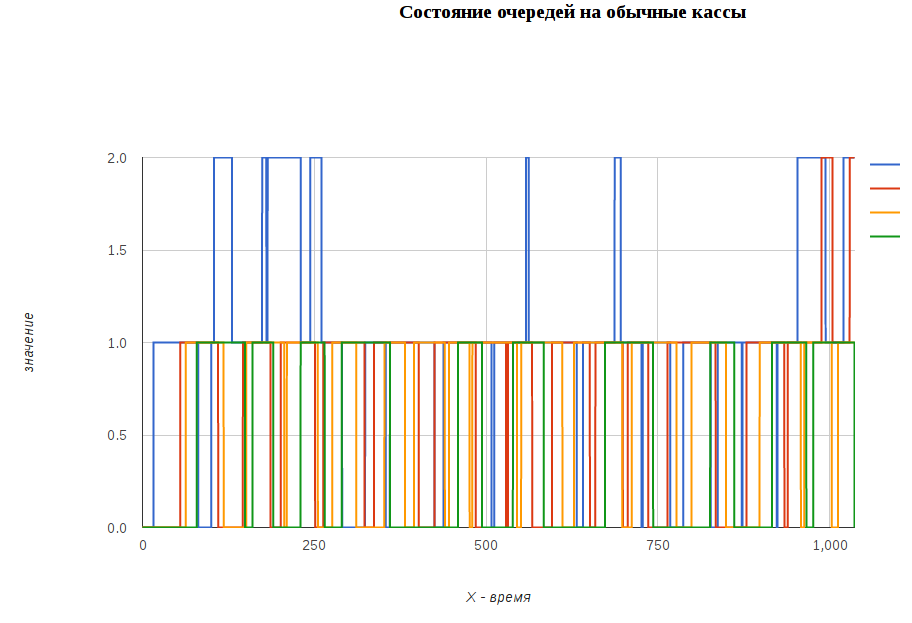
\includegraphics[scale=0.6]{screen3.png}
  \caption{Длинна очереди в каждой обычной кассе}
\end{figure}